\documentclass[11pt]{charter}

% El títulos de la memoria, se usa en la carátula y se puede usar el cualquier lugar del documento con el comando \ttitle
\titulo{Segmentación de clientes basada en aprendizaje automático} 

% Nombre del posgrado, se usa en la carátula y se puede usar el cualquier lugar del documento con el comando \degreename
%\posgrado{Carrera de Especialización en Sistemas Embebidos} 
%\posgrado{Carrera de Especialización en Internet de las Cosas} 
\posgrado{Carrera de especialización en intelegencia artificial}
%\posgrado{Maestría en Sistemas Embebidos} 
%\posgrado{Maestría en Internet de las cosas}

% Tu nombre, se puede usar el cualquier lugar del documento con el comando \authorname
\autor{Tec. David Mauricio Broin} 

% El nombre del director y co-director, se puede usar el cualquier lugar del documento con el comando \supname y \cosupname y 
%\pertesupname y \pertecosupname
\director{Ing. Yoel Yamil López}
\pertenenciaDirector{FIUBA} 
% FIXME:NO IMPLEMENTADO EL CODIRECTOR ni su pertenencia
\codirector{} % si queda vacio no se deberíá incluir 
\pertenenciaCoDirector{}

% Nombre del cliente, quien va a aprobar los resultados del proyecto, se puede usar con el comando \clientename y 
%\empclientename
\cliente{Gabriel Lourenco}
\empresaCliente{PLAYTRAK Sistemas de Monitoreo SA de CV}

% Nombre y pertenencia de los jurados, se pueden usar el cualquier lugar del documento con el comando \jurunoname, 
%\jurdosname y \jurtresname y \perteunoname, \pertedosname y \pertetresname.
\juradoUno{Nombre y Apellido (1)}
\pertenenciaJurUno{pertenencia (1)} 
\juradoDos{Nombre y Apellido (2)}
\pertenenciaJurDos{pertenencia (2)}
\juradoTres{Nombre y Apellido (3)}
\pertenenciaJurTres{pertenencia (3)}
 
\fechaINICIO{5 de marzo de 2021}		%Fecha de inicio de la cursada de GdP \fechaInicioName
\fechaFINALPlanificacion{23 de abril de 2021} 	%Fecha de final de cursada de GdP
\fechaFINALTrabajo{15 de diciembre de 2021}		%Fecha de defensa pública del trabajo final


\begin{document}

\maketitle
\thispagestyle{empty}
\pagebreak


\thispagestyle{empty}
{\setlength{\parskip}{0pt}
\tableofcontents{}
}
\pagebreak


\section{Registros de cambios}
\label{sec:registro}


\begin{table}[ht]
\label{tab:registro}
\centering
\begin{tabularx}{\linewidth}{@{}|c|X|c|@{}}
\hline
\rowcolor[HTML]{C0C0C0} 
Revisión & \multicolumn{1}{c|}{\cellcolor[HTML]{C0C0C0}Detalles de los cambios realizados} & Fecha      \\ \hline
1.0      & Creación del documento                                          & 01/04/2021 \\ \hline
1.1      & Agregar descripción                                          & 05/04/2021 \\ \hline
1.2      & Completa puntos que no dependen de WBS                       & 12/04/2021 \\ \hline
1.3      & Completa WBS, AoN y diagrama de Gantt                        & 13/04/2021 \\ \hline
1.4      & Completa seguimiento y control, gestión de riesgos y calidad & 14/04/2021 \\ \hline
\end{tabularx}
\end{table}

\pagebreak



\section{Acta de constitución del proyecto}
\label{sec:acta}

\begin{flushright}
Mendoza, \fechaInicioName
\end{flushright}

\vspace{2cm}

Por medio de la presente se acuerda con \authorname\hspace{1px} que su trabajo final de la \degreename\hspace{1px} 
se titulará ``\ttitle'', consistirá esencialmente en el prototipo preliminar de un sistema capaz de analizar el historial de 
transacciones y devolver la categoría para un cliente dado, utilizando aprendizaje automático, y tendrá un presupuesto 
preliminar estimado de 600 hs de trabajo y USD1300, con fecha de inicio \fechaInicioName\hspace{1px} y fecha de presentación 
pública \fechaFinalName.

Se adjunta a esta acta el plan inicial.

\vfill

% Esta parte se construye sola con la información que hayan cargado en el preámbulo del documento y no debe modificarla
\begin{table}[ht]
  \centering
  \begin{tabular}{ccc}
    \begin{tabular}[c]{@{}c@{}}Ariel Lutenberg \\ Director posgrado FIUBA\end{tabular} & 
    \hspace{2cm} & \begin{tabular}[c]{@{}c@{}}\clientename \\ \empclientename \end{tabular} 
    \vspace{2.5cm} \\ 
    \multicolumn{3}{c}{\begin{tabular}[c]{@{}c@{}} \supname \\ Director del Trabajo Final\end{tabular}} \vspace{2.5cm} \\
    %\begin{tabular}[c]{@{}c@{}}\jurunoname \\ Jurado del Trabajo Final\end{tabular}     &  & 
    %\begin{tabular}[c]{@{}c@{}}\jurdosname\\ Jurado del Trabajo Final\end{tabular}  \vspace{2.5cm}  \\
    %\multicolumn{3}{c}{\begin{tabular}[c]{@{}c@{}} \jurtresname\\ Jurado del Trabajo Final\end{tabular}} \vspace{.5cm}                                                                     
  \end{tabular}
\end{table}




\section{Descripción técnica-conceptual del proyecto a realizar}
\label{sec:descripcion}

PLAYTRAK Sistemas de Monitoreo es una empresa que provee soluciones para la administración y operación
de casinos. Desde sus comienzos, la compañía se esfuerza por innovar y darle a sus clientes
herramientas que faciliten, entre otros aspectos, el análisis de los datos disponibles.

Dentro de la información disponible para analizar se encuentran las transacciones de los clientes. A
través de este proyecto se busca utilizar los registros de actividad para categorizar a dichos clientes.
El objetivo es otorgar atención diferenciada y optimizar el trabajo de los colaboradores encargados de 
gestionar la cartera.

El mercado de proveedores de servicio de sistemas para casinos es bastante competitivo, por lo que imponerse
en este segmento implica no quedarse atrasado respecto a la oferta de la competencia. En este contexto, ya hay 
proveedores que tienen soluciones relacionadas con \textit{Business Intelligence} y es por esto que PLAYTRAK
decide moverse en esta dirección.

Por otro lado, el resultado de este proyecto será un \textit{software} completamente independiente a la
plataforma actual. Esto dará la flexibilidad para integrarse con otros proveedores y ser, posiblente, una
nueva forma de llegar a potenciales clientes.

En la Figura \ref{fig:context_dia} se presenta el diagrama de contexto del sistema que se propone desarrollar.
El cliente realiza diferentes actividades que son registradas por el sistema actual. Se busca entrenar al 
\textit{software} que segmentará el conjunto de clientes de tal manera que para el personal de operación 
sea trivial identificar a aquellos visitantes que mayor valor poseen para el negocio.

\vspace{25px}

\begin{figure}[htpb]
  \centering
  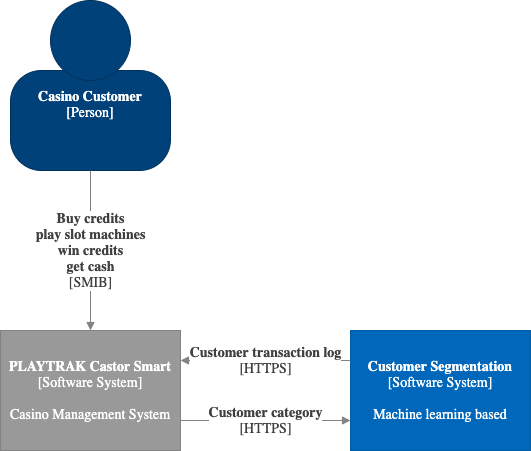
\includegraphics[width=.8\textwidth]{./Figuras/context_diagram.png}
  \caption{Diagrama de contexto del sistema propuesto}
  \label{fig:context_dia}
\end{figure}

\vspace{25px}

\section{Identificación y análisis de los interesados}
\label{sec:interesados}

\begin{table}[ht]
%\caption{Identificación de los interesados}
%\label{tab:interesados}
\begin{tabularx}{\linewidth}{@{}|l|X|X|l|@{}}
\hline
\rowcolor[HTML]{C0C0C0} 
Rol           & Nombre y Apellido & Organización 	& Puesto 	\\ \hline
Cliente       & \clientename      &\empclientename	&  Director de la empresa      	\\ \hline
Responsable   & \authorname       & FIUBA        	& Alumno 	\\ \hline
Orientador    & \supname	      & \pertesupname 	& Director	trabajo final \\ \hline
\end{tabularx}
\end{table}

\begin{itemize}
\item Cliente: sólo marca lineamientos generales y resultados a obtener, no brinda ningún tipo de detalle sobre la implementación.
\item Director: se involucra desde el principio del proyecto y es también orientador.
\end{itemize}



\section{1. Propósito del proyecto}
\label{sec:proposito}

El propósito de este proyecto es darle al cliente un nuevo producto para llegar, a su vez, a sus clientes actuales
y potenciales. Dicho producto es un sistema de segmentación de clientes que recibe compras, pagos, apuestas y ganancia; 
y devuelve categorías de usuarios.  

\section{2. Alcance del proyecto}
\label{sec:alcance}

El proyecto comprende todo el ciclo de vida de desarrollo del \textit{software}, desde el análisis hasta las herramientas
necesarias para la operación (despliegue y monitoreo).

El presente proyecto no incluye ningún tipo de trabajo sobre el actual sistema del cliente.

\section{3. Supuestos del proyecto}
\label{sec:supuestos}

Para el desarrollo del presente proyecto se supone que el cliente permitirá el desarrollo dentro de la jornada laboral.

\section{4. Requerimientos}
\label{sec:requerimientos}

\begin{enumerate}
\item Grupo de requerimientos asociados con funcionalidad
	\begin{enumerate}
	\item Interfaz REST JSON.
	\item \textit{Endpoint} POST para recibir compras por cliente.
	\item \textit{Endpoint} POST para recibir pagos por cliente.
	\item \textit{Endpoint} POST para recibir apuestas por cliente.
	\item \textit{Endpoint} POST para recibir ganancia por cliente.
	\item \textit{Endpoint} GET para recibir cliente y devolver categoría.
  \item Debe contar con configuración de GitLab CI y tener despliegue automático a AWS.
	\end{enumerate}
\item Grupo de requerimientos asociados con flujo de trabajo
	\begin{enumerate}
	\item El código fuente debe estar alojado en GitLab.
	\item Se debe implementar DevOps y el proyecto debe estar siempre disponible para revisión.
	\item El desarrollo se debe realizar usando \textit{Test Driven Development}.
	\end{enumerate}
\item Grupo de requerimientos asociados con documentación
  \begin{enumerate}
    \item La documentación debe estar escrita en \textit{markdown} y alojada usando MkDocs o similar.
    \item Debe contar con el detalle para operaciones (instalación del \textit{software}).
    \item Debe contar con el detalle de uso (información para usuarios).
    \item Debe contar con el detalle para extender las funcionalidades (información para otros programadores).
  \end{enumerate}
\end{enumerate}

\section{Historias de usuarios (\textit{Product backlog})}
\label{sec:backlog}
A continuación se listan las historias de usuario para este proyecto, entre paréntesis se encuentra el peso
de cada una de ellas. Al final de esta sección se detalla el criterio para determinar este atributo.

\begin{enumerate}
  \item Como operador de un casino quiero que el sistema clasifique los clientes en función de sus transacciones
  de caja y de juego (Cantidad: 5; complejidad: 13; riesgo: 5; total: 325).
  \item Como cliente de un casino quiero conocer mi catergoría para saber qué beneficios me corresponden (Cantidad: 3; 
  complejidad: 5; riesgo: 2; total: 30).
  \item Como operador de un casino quiero ver los clientes que están en cada categoría para poder darles 
  atención diferenciada (Cantidad: 3; complejidad: 5; riesgo: 2; total: 30).
  \item Como SMIB (\textit{Slot Machine Interface Board}) quiero conocer la categoría del cliente que está jugando 
  para poder personalizar la interfaz gráfica (Cantidad: 3; complejidad: 1; riesgo: 2; total: 6).
\end{enumerate}

A continuación se presenta el criterio para determinar \textit{storypoints}

\begin{itemize}
  \item Cantidad de trabajo a realizar.
  \begin{itemize}
    \item Bajo: 1
    \item Medio: 3
    \item Alto: 5
  \end{itemize}
  \item Complejidad del trabajo a realizar.
  \begin{itemize}
    \item Bajo: 1
    \item Medio: 5
    \item Alto: 13
  \end{itemize}
  \item Riesgo o incertidumre del trabajo a realizar
  \begin{itemize}
    \item Bajo: 2
    \item Medio: 3
    \item Alto: 5
  \end{itemize}
\end{itemize}

\section{5. Entregables principales del proyecto}
\label{sec:entregables}

\begin{itemize}
\item Repositorio/s en GitLab.
\item \textit{Software} funcionando en la nube.
\item Docuementación publicada como sitio web.
\end{itemize}

\section{6. Desglose del trabajo en tareas}
\label{sec:wbs}

\begin{enumerate}
  \item Organización. (total 90 hs)
    \begin{enumerate}
    \item Planificación del proyecto. (90 hs)
    \end{enumerate}
  \item Ejecución. (total 390 hs)
    \begin{enumerate}
    \item Análisis del problema. 
    \begin{enumerate}
      \item Identificación del problema de negocio. (30 hs)
      \item Obtener la información relevante. (30 hs)
      \item Transformar el problema de negocio en una hipótesis comprobable. (30 hs)
    \end{enumerate}
    \item Análisis exploratorio de datos. (81 hs) 
    \begin{enumerate}
      \item Visualización de datos.
      \item Prueba de hipótesis.
    \end{enumerate}
    \item Ingeniería de \textit{features} (60 hs)
    \item Prototipado (modelo de \textit{Machine Learning}) (99 hs)
    \item Ensayos y pruebas 
    \begin{enumerate}
      \item Ensayo de prototipo v1. (15 hs)
      \item Ajustes según respuesta del cliente. (30 hs)
      \item Ensayo de prototipo v2. (15 hs)
    \end{enumerate}
    \end{enumerate}
  \item Finalización (total 120 hs)
    \begin{enumerate}
      \item Primera versión de la Memoria (30 hs)
      \item Segunda versión de la Memoria (30 hs)
      \item Versión Final de la Memoria (30 hs)
      \item Elaborar la presentación (30 hs)
    \end{enumerate}
\end{enumerate}

Cantidad total de horas: (600 hs)

\section{7. Diagrama de Activity On Node}
\label{sec:AoN}

\begin{figure}[htpb]
\centering 
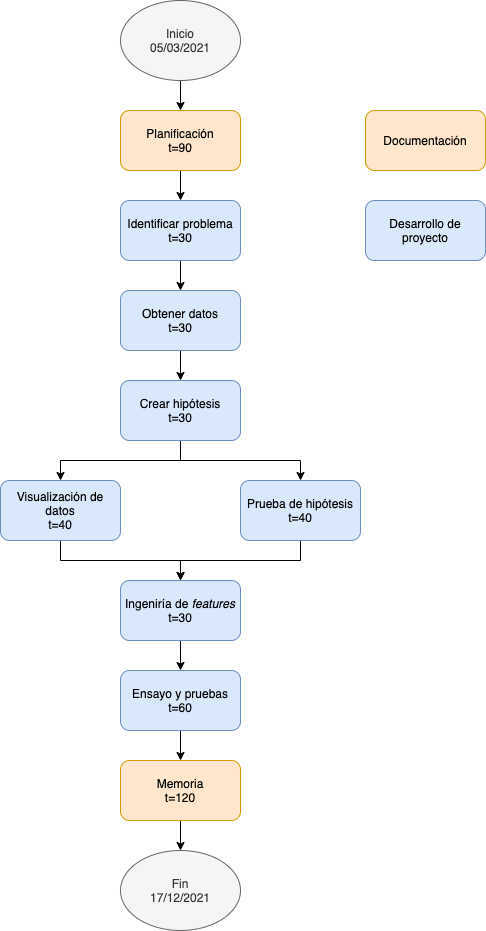
\includegraphics[width=.78\textwidth]{./Figuras/activity_on_node.png}
\caption{Diagrama en \textit{Activity on Node}}
\label{fig:AoN}
\end{figure}

Los tiempos están expresados en horas.

\section{8. Diagrama de Gantt}
\label{sec:gantt}

\begin{figure}[htpb]
  \begin{ganttchart}[
    time slot unit=day,
    time slot format=isodate,
    x unit=0.038cm,
    y unit title=0.7cm,
    y unit chart=0.6cm,
    milestone/.append style={xscale=4}
    ]{2021-03-5}{2021-12-17}
    \gantttitlecalendar*{2021-03-5}{2021-12-17}{year} \\
    \gantttitlecalendar*{2021-03-5}{2021-12-17}{month} \\
    \ganttgroup{Duración Total}{2021-03-5}{2021-12-17} \\
    %%%%%%%%%%%%%%%%%Organización
    \ganttgroup{Organización}{2021-03-5}{2021-04-16} \\
    \ganttbar{Planificación del proyecto}{2021-03-5}{2021-04-16} \\
    %%%%%%%%%%%%%%%%%Ejecución
    \ganttgroup{Ejecución}{2021-04-19}{2021-10-15} \\
    \ganttbar{Identificación del problema}{2021-04-19}{2021-04-30} \\
    \ganttbar{Obtener la información}{2021-05-3}{2021-05-14} \\
    \ganttbar{Hipótesis comprobable}{2021-05-17}{2021-05-28} \\
    \ganttbar{Visualización de datos}{2021-05-31}{2021-07-14} \\
    \ganttbar{Prueba de hipótesis}{2021-05-31}{2021-07-14} \\
    \ganttbar{Ingeniería de \textit{features}}{2021-07-15}{2021-08-11} \\
    \ganttbar{Prototipado}{2021-08-12}{2021-09-24} \\
    \ganttbar{Ensayo de prototipo v1}{2021-09-27}{2021-10-1} \\
    \ganttbar{Ajustes según respuesta}{2021-10-4}{2021-10-15} \\
    \ganttbar{Ensayo de prototipo v2}{2021-10-18}{2021-10-22} \\
    % %%%%%%%%%%%%%%%%%Finalización
    \ganttgroup{Finalización}{2021-10-25}{2021-12-17} \\
    \ganttbar{Memoria v1}{2021-10-25}{2021-11-5} \\
    \ganttbar{Memoria v2}{2021-11-8}{2021-11-19} \\
    \ganttbar{Memoria final}{2021-11-22}{2021-12-3} \\
    \ganttmilestone{Enviar memoria al director}{2021-12-3} \\
    \ganttbar{Elaborar la presentación}{2021-12-6}{2021-12-17} \\
    \ganttmilestone{Ensayo de la presentación}{2021-12-17} \\
    %%%%%%%%%%%%%%%%%%%%%%%%%%%%%%%%%%%%%%%%%%%%%%%%%%%%%%%%%%%%%%%
  \end{ganttchart}
  \caption{Diagrama de Gantt.}
  \label{fig:gantt}
\end{figure}

\section{9. Matriz de uso de recursos de materiales}
\label{sec:recursos}


\begin{table}[htpb]
\label{tab:recursos}
\centering
\begin{tabularx}{\linewidth}{@{}|c|X|X|X|X|c|@{}}
\hline
\cellcolor[HTML]{C0C0C0} & \cellcolor[HTML]{C0C0C0} & \multicolumn{3}{c|}{\cellcolor[HTML]{C0C0C0}Recursos requeridos (horas)} \\ \cline{3-5} 
\multirow{-2}{*}{\cellcolor[HTML]{C0C0C0}\begin{tabular}[c]{@{}c@{}}Código\\ WBS\end{tabular}} & \multirow{-2}{*}{\cellcolor[HTML]{C0C0C0}\begin{tabular}[c]{@{}c@{}}Nombre \\ tarea\end{tabular}} & Laptop & Lugar de trabajo & Infrastrutura \textit{cloud} \\ \hline
1 & Proyecto final & 600 & 600 & 600 \\ \hline

\end{tabularx}%
\end{table}


\section{10. Presupuesto detallado del proyecto}
\label{sec:presupuesto}

A continuación se detallan los costos del proyecto en dólares estadounidenses.

\begin{table}[htpb]
  \centering
  \begin{tabularx}{\linewidth}{@{}|X|c|r|r|@{}}
  \hline
  \rowcolor[HTML]{C0C0C0} 
  \multicolumn{4}{|c|}{\cellcolor[HTML]{C0C0C0}COSTOS DIRECTOS} \\ \hline
  \rowcolor[HTML]{C0C0C0} 
  Descripción &
  \multicolumn{1}{c|}{\cellcolor[HTML]{C0C0C0}Cantidad} &
  \multicolumn{1}{c|}{\cellcolor[HTML]{C0C0C0}Valor unitario} &
  \multicolumn{1}{c|}{\cellcolor[HTML]{C0C0C0}Valor total} \\ \hline
Profesionales (salario bruto) &
  12 &
  5000 &
  60000 \\ \hline
Oficina equipada &
  12 &
  400 &
  4800 \\ \hline
Servicios externos de administración &
  12 &
  600 &
  7200 \\ \hline
Infraestructura \textit{cloud} &
  12 &
  28 &
  336 \\ \hline
Laptop &
  12 &
  69.44 &
  833.33 \\ \hline
Sistemas Informáticos (Google Workspace) &
  12 &
  5 &
  60 \\ \hline
\multicolumn{3}{|c|}{SUBTOTAL} &
  73.229,33 \\ \hline
  \rowcolor[HTML]{C0C0C0} 
  \multicolumn{4}{|c|}{\cellcolor[HTML]{C0C0C0}COSTOS INDIRECTOS} \\ \hline
  \rowcolor[HTML]{C0C0C0} 
  Descripción &
    \multicolumn{1}{c|}{\cellcolor[HTML]{C0C0C0}Cantidad} &
    \multicolumn{1}{c|}{\cellcolor[HTML]{C0C0C0}Valor unitario} &
    \multicolumn{1}{c|}{\cellcolor[HTML]{C0C0C0}Valor total} \\ \hline
  \multicolumn{1}{|l|}{30\% de los costos directos} &
    1 &
    24.165,68 &
    24.165,68 \\ \hline
  \rowcolor[HTML]{C0C0C0}
  \multicolumn{3}{|c|}{TOTAL} &
    97.395,01 \\ \hline
  \end{tabularx}%
  \end{table}


\section{11. Matriz de asignación de responsabilidades}
\label{sec:responsabilidades}

\begin{table}[htpb]
\centering
\resizebox{\textwidth}{!}{%
\begin{tabular}{|c|c|c|c|c|}
\hline
\rowcolor[HTML]{C0C0C0} 
\cellcolor[HTML]{C0C0C0} &
  \cellcolor[HTML]{C0C0C0} &
  \multicolumn{3}{c|}{\cellcolor[HTML]{C0C0C0}Listar todos los nombres y roles del proyecto} \\ \cline{3-5} 
\rowcolor[HTML]{C0C0C0} 
\cellcolor[HTML]{C0C0C0} &
  \cellcolor[HTML]{C0C0C0} &
  Responsable &
  Orientador &
  % Equipo &
  Cliente \\ \cline{3-5} 
\rowcolor[HTML]{C0C0C0} 
\multirow{-3}{*}{\cellcolor[HTML]{C0C0C0}\begin{tabular}[c]{@{}c@{}}Código\\ WBS\end{tabular}} &
  \multirow{-3}{*}{\cellcolor[HTML]{C0C0C0}Nombre de la tarea} &
  \authorname &
  \supname &
  % Nombre de alguien & 
  \clientename \\ \hline
1.1   & Planificación del proyecto. & P & C & A \\ \hline
2.1.1 & Identificación del problema. & P & C & A \\ \hline
2.1.2 & Obtener la información. & P & C & A \\ \hline
2.1.3 & Crear hipótesis. & P & C & A \\ \hline
2.2.1 & Visualización de datos. & P & C & A \\ \hline
2.2.1 & Prueba de hipótesis. & P & C & A \\ \hline
2.3   & Ingeniería de \textit{features} & P & C & A \\ \hline
2.4   & Prototipado & P & C & A \\ \hline
2.5.1 & Ensayo de prototipo v1. & P & I & A \\ \hline
2.5.2 & Ajustes según respuesta. & P & I & A \\ \hline
2.5.3 & Ensayo de prototipo v2. & P & I & A \\ \hline
3.1   & Memoria v1 & P & C &  \\ \hline
3.2   & Memoria v2 & P & C &  \\ \hline
3.3   & Versión Final de la Memoria & P & A &  \\ \hline
3.4   & Elaborar la presentación & P & I &  \\ \hline
\end{tabular}%
}
\end{table}

{\footnotesize
Referencias:
\begin{itemize}
	\item P = Responsabilidad Primaria
	\item S = Responsabilidad Secundaria
	\item A = Aprobación
	\item I = Informado
	\item C = Consultado
\end{itemize}
} %footnotesize

\section{12. Gestión de riesgos}
\label{sec:riesgos}

\begin{itemize}
  \item Riesgo 1: Suspensión definitiva de la actividad de PLAYTRAK por contingencia sanitaria.
  \begin{itemize}
    \item Severidad (9): La interrupción de la actividad de la empresa auspiciante, pondría en riesgo la 
    continuidad del proyecto.
    \item Ocurrencia (8): Durante el año pasado esto sucedió y es posible que vuelva a suceder.
  \end{itemize}
\end{itemize}

\begin{itemize}
  \item Riesgo 2: Imposibilidad de la empresa de permitir el desarrollo en horario laboral.
  \begin{itemize}
    \item Severidad (5): No sería tan grave porque se podría intentar continuar con el desarrollo fuera del 
    horario laboral. Esto probablemente dilataría el trabajo en el tiempo, pero se podría concretar.
    \item Ocurrencia (9): No es prioritario para la compañía la incorporación de intelegencia artificial.
  \end{itemize}
\end{itemize}

\begin{itemize}
  \item Riesgo 3: Imposibilidad de seguir esta planificación
  \begin{itemize}
    \item Severidad (10): En este caso, la empresa cancelaría el proyecto. Este proyecto se mantiene en pie por 
    la importancia académica.
    \item Ocurrencia (7): A la hora de armar esta planificación no se tiene experiencia en el desarrollo
    de proyectos de este tipo, por lo que se esperan variaciones.
  \end{itemize}
\end{itemize}

\begin{itemize}
  \item Riesgo 4: Fracaso de la usabilidad de este proyecto
  \begin{itemize}
    \item Severidad (8): El cliente plantea este proyecto a modo de prototipo de un producto que le permitiría mejorar 
    la atención a clientes. Es posible que PLAYTRAK, más allá de haber puesto esfuerzo en esta planificación, 
    determine que no es factible implementar este producto. Si se detecta esto en medio del avance del proyecto, 
    puede llegar a ser cancelado.
    \item Ocurrencia (3): Durante la elaboración de la planificación se ha repasado ampliamente el 
    valor que este proyecto le ofrece al sistema de administración de casinos que PLAYTRAK ofrece.
  \end{itemize}
\end{itemize}
 
\begin{itemize}
  \item Riesgo 5: Pérdida material o rotura del equipo de cómputo
  \begin{itemize}
    \item Severidad (6): Tal como se muestra en el apartado (9), la computadora es el recurso más utilizado en este proyecto. 
    La severidad se ve disminuida por el hecho de que se podría conseguir un equipo de reemplazo.
    \item Ocurrencia (1): La computadora disponible para el desarrollo de este proyecto tiene una antigüedad 
    de menos de 1 año y aún está en garantía.
  \end{itemize}
\end{itemize}

b) Tabla de gestión de riesgos:      (El RPN se calcula como RPN=SxO)

\begin{table}[htpb]
\centering
\begin{tabularx}{\linewidth}{@{}|X|c|c|c|c|c|c|@{}}
\hline
\rowcolor[HTML]{C0C0C0} 
Riesgo & S & O & RPN & S* & O* & RPN* \\ \hline
Suspensión de la actividad por contingencia sanitaria & 9  & 8 & 72  & 4 & 8 & 32  \\ \hline
Imposibilidad de desarrollar en horario laboral & 5  & 9 & 45  & 3 & 9 & 27  \\ \hline
Imposibilidad de seguir esta planificación & 10 & 7 & 70  & 3 & 7 & 21  \\ \hline
Fracaso de la usabilidad de este proyecto & 8  & 3 & 24  &   &   &     \\ \hline
Pérdida material o rotura del equipo de cómputo & 6  & 1 & 6   &   &   &     \\ \hline
\end{tabularx}%
\end{table}

Criterio adoptado: 
Se tomarán medidas de mitigación en los riesgos cuyos números de RPN sean mayores a 40.

Nota: los valores marcados con (*) en la tabla corresponden luego de haber aplicado la mitigación.

c) Plan de mitigación de los riesgos que originalmente excedían el RPN máximo establecido:

\begin{itemize}
  \item Riesgo 1: Contar con recursos económicos para poder continuar con el trabajo a pesar de no estar trabajando.
  \begin{itemize}
    \item Severidad (4): Si la empresa suspende las actividades en un estadío temprano del proeycto, se
    requiere mucho dinero para dedicar tiempo a finalizar. Si esto sucede cerca del final, se podrá concluir
    antes de buscar un nuevo trabajo.
    \item Ocurrencia (8):  No cambia con la mitigación, no es posible trabajar sobre esto.
  \end{itemize}
\end{itemize}

\begin{itemize}
  \item Riesgo 2: Dedicar tiempo fuera del trabajo al desarrollo de este proyecto.
  \begin{itemize}
    \item Severidad (3): El reponsable cuenta con tiempo extra y el proyecto se puede extender hasta
    2 años sin afectar académicamente.
    \item Ocurrencia (9): No es prioritario para la compañía la incorporación de intelegencia artificial.
  \end{itemize}
\end{itemize}

\begin{itemize}
  \item Riesgo 3: Misma mitigación que Riesgo 2.
  \begin{itemize}
    \item Severidad (3): Idem a severidad de Riesgo 2.
    \item Ocurrencia (7): A la hora de armar esta planificación no se tiene experiencia en el desarrollo
    de proyectos de este tipo, por lo que se esperan variaciones.
  \end{itemize}
\end{itemize}


\section{13. Gestión de la calidad}
\label{sec:calidad}

\begin{itemize} 
\item Req \#1: Debe recibir compras, pagos, apuestas y ganancia; y devolver categoría.

Verificación y validación:
\begin{itemize}
  \item Verificación: diseño de API con dichos parámetros de entrada. 
  \item Validación: recibir datos de clientes y devolver la categoría esperada.
\end{itemize}

\item Req \#2: El código fuente debe estar alojado en GitLab.

Verificación y validación:
\begin{itemize}
  \item Verificación: utilizar GitLab como servidor de control de versiones git.
  \item Validación: compartir el repositorio con el cliente.
\end{itemize}

\item Req \#3: Se debe implementar DevOps y el proyecto debe estar siempre disponible para revisión.

Verificación y validación:
\begin{itemize}
  \item Verificación: agregar CI/CD al repositorio.
  \item Validación: probar sobre el sitio web automáticamente desplegado.
\end{itemize}

\item Req \#4: El desarrollo se debe realizar usando \textit{Test Driven Development}.

Verificación y validación:
\begin{itemize}
  \item Verificación: escribir pruebas unitarias a priori.
  \item Validación: mostrar las pruebas unitarias pasando antes de cada despliegue. 
\end{itemize}

\item Req \#5: La documentación debe estar escrita en \textit{markdown} y alojada usando MkDocs o similar.

Verificación y validación:
\begin{itemize}
  \item Verificación: escribir la documentación en dicho lenguaje.
  \item Validación: mostrar sitio web de documentación funcionando.
\end{itemize}

\item Req \#6: Debe contar con el detalle para operaciones (instalación del \textit{software}).

Verificación y validación:
\begin{itemize}
  \item Verificación: desde el principio agregar las instrucciones para poner a funcionar el \textit{software}
  en un ambiente productivo. 
  \item Validación: tomar las instrucciones e instalar en un ambiente que cumpla con los prerequisitos.  
\end{itemize}

\item Req \#7: Debe contar con el detalle de uso (información para usuarios).

Verificación y validación:
\begin{itemize}
  \item Verificación: mantener la documentación sobre el uso con suficiente claridad.
  \item Validación: una persona sin conocimiento previo debe poder usar el \textit{software} tras leer el manual.
\end{itemize}

\item Req \#8: Debe contar con el detalle para extender las funcionalidades (información para otros programadores).

Verificación y validación:
\begin{itemize}
  \item Verificación: docuemntar la plataforma de desarrollo.
  \item Validación: un programador debe poder entender cómo extender y mantener con el \textit{software}.
\end{itemize}

\end{itemize}

\section{14. Comunicación del proyecto}
\label{sec:comunicaciones}

El plan de comunicación del proyecto es el siguiente:

\begin{table}[htpb]
  \centering
  \begin{tabularx}{\linewidth}{@{}|X|C{2.4cm}|C{3cm}|C{1.8cm}|C{2cm}|C{2.1cm}|@{}}
  \hline
  \rowcolor[HTML]{C0C0C0} 
  \multicolumn{6}{|c|}{\cellcolor[HTML]{C0C0C0}PLAN DE COMUNICACIÓN DEL PROYECTO}           \\ \hline
  \rowcolor[HTML]{C0C0C0} 
  ¿Qué comunicar? & Audiencia & Propósito & Frecuencia & Método de comunicac. & Responsable \\ \hline
  Plan de Trabajo               & Alumnos y docentes \newline Gestión de Proyectos & Dar a conocer el proyecto y la planificación                                            & Única vez            & Videoconferencia     & David Broin \\ \hline
  Avance de Proyecto            & Cliente                                                                            & Seguimiento del trabajo                                                                 & Diario               & Chat                 & David Broin \\ \hline
  Avance de Proyecto            & Director del trabajo final                                                         & Seguimiento del trabajo                                                                 & Mensual              & Correo Electrónico   & David Broin \\ \hline
  Informe de avance             & Jurados                                                                            & Mostrar avance del trabajo                                                              & Única vez            & Correo Electrónico   & David Broin \\ \hline
  Problemas de costos y alcance & Director del Trabajo y docentes de la carrera                                      & Advertir sobre problemas con el cliente que ponen en riesgo la continuidad del proyecto & Cuando sea necesario & Correo Electrónico   & David Broin \\ \hline
  Memoria de Proyecto Final     & Jurados y Director del trabajo final                                               & Presentación para su evaluación y aprobación                                            & Única vez            & Correo Electrónico   & David Broin \\ \hline
  \end{tabularx}
\end{table}

\section{15. Gestión de compras}
\label{sec:compras}

Criterios para elección de proveedor:
\begin{itemize}
  \item El precio más bajo (se solicita cotización a 3 proveedores)
  \item Disposición inmediata de los servicios.
  \item Se comienza cotizando los servicios a los proveedores conocidos por el cliente.
  \item Las compras se realizan por internet y pago directo con tarjeta de crédito.
\end{itemize}

\section{16. Seguimiento y control}
\label{sec:seguimiento}

\begin{table}[!htpb]
\centering
%\begin{tabularx}{\linewidth}{@{}|X|X|X|X|X|X|@{}}
\begin{tabularx}{\linewidth}{@{}|X|C{2.5cm}|C{3cm}|C{2cm}|C{2cm}|C{2.5cm}|@{}}
\hline
\rowcolor[HTML]{C0C0C0} 
\multicolumn{6}{|c|}{\cellcolor[HTML]{C0C0C0}SEGUIMIENTO DE AVANCE}                                                                       \\ \hline
\rowcolor[HTML]{C0C0C0} 
Tarea del WBS & Indicador de avance & Frecuencia de reporte & Resp. de seguimiento & Persona a ser informada & Método de comunic. \\ \hline
1.1   & Sección completada & Semanal & David Broin & Patricio Boss & Google Forms \\ \hline
2.1.1 & Tareas en issue & Única vez & David Broin & Gabriel Lourenco & Merge Request GitLab \\ \hline
2.1.2 & Tareas en issue & Única vez & David Broin & Gabriel Lourenco & Merge Request GitLab \\ \hline
2.1.3 & Tareas en issue & Única vez & David Broin & Gabriel Lourenco & Merge Request GitLab \\ \hline
2.2.1 & Tareas en issue & Única vez & David Broin & Gabriel Lourenco & Merge Request GitLab \\ \hline
2.2.1 & Tareas en issue & Única vez & David Broin & Gabriel Lourenco & Merge Request GitLab \\ \hline
2.3   & Tareas en issue & Única vez & David Broin & Gabriel Lourenco & Merge Request GitLab \\ \hline
2.4   & Tareas en issue & Única vez & David Broin & Gabriel Lourenco & Merge Request GitLab \\ \hline
2.5.1 & Tareas en issue & Única vez & David Broin & Gabriel Lourenco & Merge Request GitLab \\ \hline
2.5.2 & Tareas en issue & Única vez & David Broin & Gabriel Lourenco & Merge Request GitLab \\ \hline
2.5.3 & Tareas en issue & Única vez & David Broin & Gabriel Lourenco & Merge Request GitLab \\ \hline
3.1   & Sección completada & Única vez & David Broin & Docente & Google Forms \\ \hline
3.2   & Sección completada & Única vez & David Broin & Docente & Google Forms \\ \hline
3.3   & Sección completada & Única vez & David Broin & Director del Trabajo Final & Correo electrónico \\ \hline
3.4   & Documento terminado & Única vez & David Broin & Docente & Correo electrónico \\ \hline
\end{tabularx}%
%}
\end{table}

\section{17. Procesos de cierre}    
\label{sec:cierre}

Establecer las pautas de trabajo para realizar una reunión final de evaluación del proyecto, tal que contemple las 
siguientes actividades:

\begin{itemize}
\item Pautas de trabajo que se seguirán para analizar si se respetó el Plan de Proyecto original:
\begin{itemize}
  \item Responsable: David Broin
  \item Se evaluarán:
  \begin{itemize}
    \item Requisitos: se tienen que cumplir los enumerados en este plan de trabajo.
    \item Fechas de las entregas al cliente. 
  \end{itemize}
\end{itemize}
\item Identificación de las técnicas y procedimientos útiles e inútiles que se emplearon, y los problemas que surgieron 
y cómo se solucionaron:
\begin{itemize}
  \item Responsable: David Broin
  \item Se evaluarán:
  \begin{itemize}
    \item Los procedimientos y técnicas que se reconocen fácilmente como positivos para lograr objetivo requerido 
    por el cliente.
    \item Los procedimientos y técnicas que entorpecieron el desarrollo, pero que se reconoce que son útiles.
    \item Los procedimientos y técnicas que no ofrecieron ningún tipo de valor al proyecto.
  \end{itemize}
\end{itemize}
\item Indicar quién organizará el acto de agradecimiento a todos los interesados, y en especial al equipo de trabajo 
y colaboradores:
  \begin{itemize}
    \item Responsable: David Broin
    \item El responsable del proyecto invita formalmente a todas las personas que aportaron e hicieron posible 
    la realización del proyecto.
  \end{itemize}
\end{itemize}

\end{document}
